%%%%%%%%%%%%%%%%%%%%%%%%%%%%%%%%%%%%%%%%%%%%%%%%%%%%%%%%%%%%%%%%%%%%%%%%%%%

\documentclass{standalone}

\usepackage{amsmath}
\usepackage{mathptmx}
\usepackage{pgfplots}
\usetikzlibrary{external}
\tikzexternalize{sunflower}
\pgfplotsset{compat=1.16}

%% IEEE uses Times Roman font, so we'll default to Times.
%% These three commands make up the entire times.sty package.
\renewcommand{\rmdefault}{ptm}
\renewcommand{\ttdefault}{pcr}
\normalfont\selectfont

\begin{document}

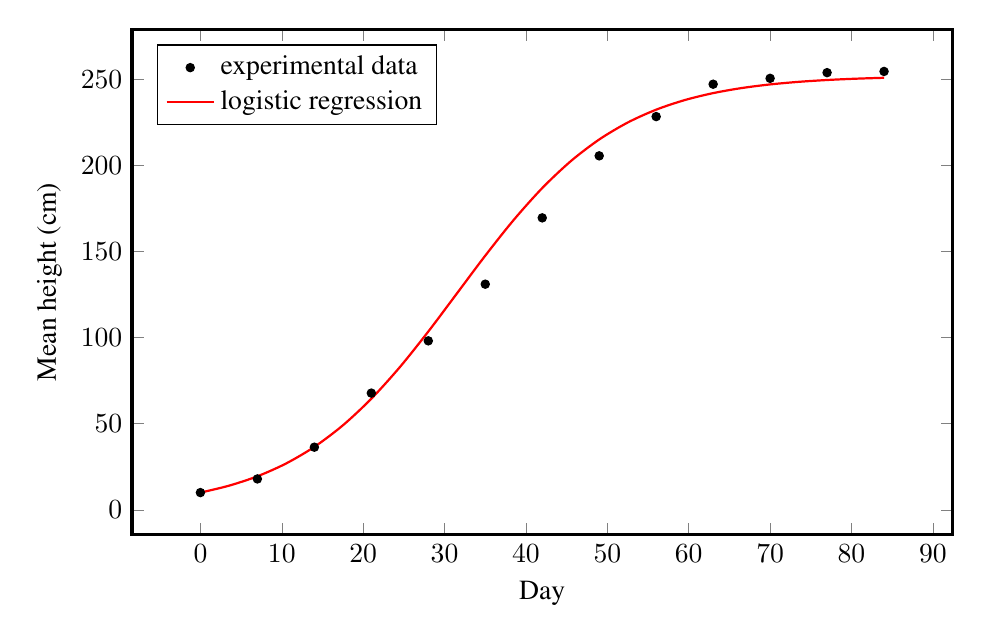
\begin{tikzpicture}
\tikzset{%%
  every mark/.append style={scale=1.0},%%
  scale=1.0%%
}
\pgfplotsset{%%
  every axis/.append style={font=\normalsize}%%
}
%%
\begin{axis}[%%
  axis line style=very thick,%%
  dotStyle/.style={mark size=1.5,black,mark color=black,mark=*,only marks},%%
  enlargelimits=true,%%
  height=8cm,%%
  legend cell align=left,%%
  legend pos=north west,%%
  plotStyle/.style={%%
    domain=0:84,%%
    mark=none,%%
    smooth,%%
    thick%%
  },%%
  width=12cm,%%
  %% x axis
  xlabel={\normalsize Day},%%
  %% y axis
  ylabel={\normalsize Mean height~(cm)}%%
]
%%
%%
\addplot[dotStyle] coordinates {
  (0, 10)
  (7, 17.93)
  (14, 36.36)
  (21, 67.76)
  (28, 98.1)
  (35, 131)
  (42, 169.5)
  (49, 205.5)
  (56, 228.3)
  (63, 247.1)
  (70, 250.5)
  (77, 253.8)
  (84, 254.5)
};
\addlegendentry{experimental data}
%%
%%
\addplot+ [plotStyle,red]
{252.0837 / (1 + 24.2083 * exp(-0.1009*x))};
\addlegendentry{logistic regression}
\end{axis}
\end{tikzpicture}

\end{document}
